\documentclass[tikz,border=2pt]{standalone}
\usepackage{amsmath,amssymb}
\usepackage{tikz}
\usetikzlibrary{arrows.meta}

\begin{document}
% The event generated by X and B is the preimage {omega : X(omega) in B}: pull the set B on
% the real line back to the sample space.
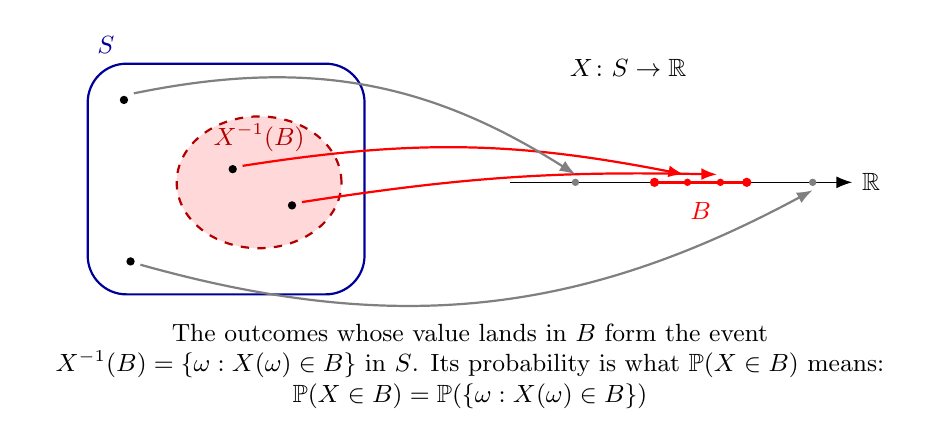
\begin{tikzpicture}[scale=0.837,   every node/.style={font=\small}, >={Latex[length=2mm]}]
	\draw[thick, blue!60!black, rounded corners=14pt] (-2.0,-1.7) rectangle (2.2,1.8);
	\node[blue!60!black, anchor=south west] at (-2.0,1.8) {$S$};
	\fill[red!15] (0.6,0.0) ellipse (1.25 and 1.0);
	\draw[red!70!black, thick, dashed] (0.6,0.0) ellipse (1.25 and 1.0);
	\node[red!70!black, font=\small] at (0.6,0.68) {$X^{-1}(B)$};
	\fill (0.2,0.2) circle (1.8pt);
	\fill (1.1,-0.35) circle (1.8pt);
	\fill (-1.45,1.25) circle (1.8pt);
	\fill (-1.35,-1.2) circle (1.8pt);
	\draw[->] (4.4,0) -- (9.6,0) node[right] {$\mathbb{R}$};
	\draw[red, very thick] (6.6,0) -- (8.0,0);
	\fill[red] (6.6,0) circle (2pt);
	\fill[red] (8.0,0) circle (2pt);
	\node[red, anchor=north] at (7.3,-0.15) {$B$};
	\draw[->, red, thick] (0.35,0.25) to[bend left=10] (7.05,0.12);
	\draw[->, red, thick] (1.25,-0.3) to[bend left=5] (7.55,0.12);
	\draw[->, gray, thick] (-1.3,1.35) to[bend left=22] (5.4,0.12);
	\draw[->, gray, thick] (-1.2,-1.25) to[bend right=22] (9.0,-0.12);
	\fill[red] (7.1,0) circle (1.6pt);
	\fill[red] (7.6,0) circle (1.6pt);
	\fill[gray] (5.4,0) circle (1.6pt);
	\fill[gray] (9.0,0) circle (1.6pt);
	\node[anchor=south] at (6.2,1.45) {$X\colon S\to\mathbb{R}$};
	\node[anchor=north, align=flush center, text width=11cm] at (3.8,-2.0) {The outcomes whose value lands in $B$ form the event $X^{-1}(B)=\{\omega:X(\omega)\in B\}$ in $S$. Its probability is what $\mathbb{P}(X\in B)$ means: $\mathbb{P}(X\in B)=\mathbb{P}(\{\omega:X(\omega)\in B\})$};
\end{tikzpicture}
\end{document}
